%%%%%%%%%%%%%%%%%%%%%%%%%%%%%%%%%%%%%%%%%%%%%%%%%%%%%%%%%%%%
%%  This Beamer template was created by Cameron Bracken.
%%  Anyone can freely use or modify it for any purpose
%%  without attribution.
%%
%%  Last Modified: January 9, 2009
%%

\documentclass[xcolor=x11names,compress]{beamer}

%% General document %%%%%%%%%%%%%%%%%%%%%%%%%%%%%%%%%%
\usepackage{graphicx}
\usepackage{tikz}
\usepackage[canadian]{babel}
\usepackage[utf8]{inputenc}
\usepackage{amsmath,amssymb}
\usepackage{mathtools}
\usepackage[ruled,vlined,linesnumbered]{algorithm2e}
\usepackage{epstopdf}
\usepackage{hyperref}
\usepackage[export]{adjustbox}
\usepackage{animate}
\usepackage{minted}
\usepackage{xcolor}
\usepackage{pgfplots}
\usetikzlibrary{calc}
\graphicspath{{img/}}
%%%%%%%%%%%%%%%%%%%%%%%%%%%%%%%%%%%%%%%%%%%%%%%%%%%%%%

\DeclareMathOperator*{\argmax}{arg\,max}
\DeclareMathOperator*{\argmin}{arg\,min}
%% Beamer Layout %%%%%%%%%%%%%%%%%%%%%%%%%%%%%%%%%%
\useoutertheme[subsection=false,shadow]{miniframes}
\useinnertheme{default}
\usefonttheme{serif}
\usepackage{palatino}
\urlstyle{same}
\setbeamerfont{title like}{shape=\scshape}
\setbeamerfont{frametitle}{shape=\scshape}

\setbeamercolor*{lower separation line head}{bg=DeepSkyBlue4} 
\setbeamercolor*{normal text}{fg=black,bg=white} 
\setbeamercolor*{alerted text}{fg=red} 
\setbeamercolor*{example text}{fg=black} 
\setbeamercolor*{structure}{fg=black} 
 
\setbeamercolor*{palette tertiary}{fg=black,bg=black!10} 
\setbeamercolor*{palette quaternary}{fg=black,bg=black!10} 

\renewcommand{\(}{\begin{columns}}
\renewcommand{\)}{\end{columns}}
\newcommand{\<}[1]{\begin{column}{#1}}
\renewcommand{\>}{\end{column}}
\setbeamertemplate{navigation symbols}{}

\setbeamerfont{footline}{size=\fontsize{6}{0}\selectfont}
\setbeamercolor{footline}{fg=black!50}

\setbeamertemplate{footline}{
	\parbox{\paperwidth}{\hspace*{5pt}\url{http://www.cs.toronto.edu/~frossard}\hfill
		\insertframenumber/\inserttotalframenumber\hspace*{5pt}}
	}
\usemintedstyle{tango}
%%%%%%%%%%%%%%%%%%%%%%%%%%%%%%%%%%%%%%%%%%%%%%%%%%

\begin{document}
%%%%%%%%%%%%%%%%%%%%%%%%%%%%%%%%%%%%%%%%%%%%%%%%%%%%%%
%%%%%%%%%%%%%%%%%%%%%%%%%%%%%%%%%%%%%%%%%%%%%%%%%%%%%%
\section{\scshape Introduction}
\begin{frame}
\title{Introduction to Machine Learning}
\subtitle{Logistic Regression and Neural Networks}
\author{
Davi Frossard\\
{\it Federal University of Espirito Santo \\ University of Toronto}\\
}
\date{
\vspace{-2em}\\
\includegraphics[width=0.5\columnwidth]{cover}\\[-1ex]
{\tiny Credit: {\itshape \url{http://bit.ly/2cQtv6N}}}
\\
\today
}
\titlepage
\end{frame}

%%%%%%%%%%%%%%%%%%%%%%%%%%%%%%%%%%%%%%%%%%%%%%%%%%%%%%
%%%%%%%%%%%%%%%%%%%%%%%%%%%%%%%%%%%%%%%%%%%%%%%%%%%%%%
\begin{frame}{Summary}
\tableofcontents
\end{frame}

%%%%%%%%%%%%%%%%%%%%%%%%%%%%%%%%%%%%%%%%%%%%%%%%%%%%%%
%%%%%%%%%%%%%%%%%%%%%%%%%%%%%%%%%%%%%%%%%%%%%%%%%%%%%%
\section{\scshape Classification}
\begin{frame}{Classification}
\begin{itemize}
\item Remember the KNN class.
\item Given the input data, we want to predict what is the most likely label.
    \begin{itemize}
    	\item Match the face to the person, the handwritten digit to a number, etc.
    \end{itemize}
\item Geometrically, we want to find hyperplanes that separate the data belonging to each label.
\end{itemize}
\begin{center}
\includegraphics[width=0.35\columnwidth]{hyperplane}
\end{center}
\end{frame}

%%%%%%%%%%%%%%%%%%%%%%%%%%%%%%%%%%%%%%%%%%%%%%%%%%%%%%
%%%%%%%%%%%%%%%%%%%%%%%%%%%%%%%%%%%%%%%%%%%%%%%%%%%%%%
\section{\scshape Logistic Regression}
\begin{frame}{Logistic Regression}
\begin{itemize}
\item We've already seen KNN, which can be used for classification.
\item Another method is \textbf{Logistic Regression}, which is (loosely) an extension of Linear Regression.
\item Whereas in Linear Regression our output was simply $y = w^Tx$, it now becomes $y = \sigma\left(w^Tx\right)$, where $\sigma(x)$ is a non-linear function such as the sigmoid.
\end{itemize}
\begin{center}
\includegraphics[width=0.6\columnwidth]{sigmoid}\\[-1ex]
{\tiny Credit: {\itshape \url{http://www.saedsayad.com/artificial_neural_network.htm}}}
\end{center}
\end{frame}

%%%%%%%%%%%%%%%%%%%%%%%%%%%%%%%%%%%%%%%%%%%%%%%%%%%%%%
%%%%%%%%%%%%%%%%%%%%%%%%%%%%%%%%%%%%%%%%%%%%%%%%%%%%%%
\begin{frame}{Logistic Regression}
\begin{center}
\animategraphics[controls,width=0.7\linewidth]{12}{lr_anim/lr-}{0}{47}
\end{center}
\end{frame}



%%%%%%%%%%%%%%%%%%%%%%%%%%%%%%%%%%%%%%%%%%%%%%%%%%%%%%
%%%%%%%%%%%%%%%%%%%%%%%%%%%%%%%%%%%%%%%%%%%%%%%%%%%%%%
\subsection{Cross Entropy}
\begin{frame}{Cross Entropy}
\begin{itemize}
\item Before we can dive into Logistic Regression we must first discuss adequate cost functions.
\item Using the mean square error is a bad idea in this case.
    \only<2>{
    	\begin{itemize}
    		\item \textbf{Why?}
    	\end{itemize}
    }
    \visible<3->{
    	\item MSE pulls the model towards the mean values while in classification we want to be as sure as possible of a single label.
    	      \begin{itemize}
    	      	\item An autonomous vehicle trained using MSE when in doubt between turning left or right would just go straight.
    	      \end{itemize}
    	      \begin{center}
    	      	\includegraphics[width=0.4\columnwidth]{crash}\\[-1ex]
    	      	{\tiny Credit: {\itshape \url{http://menaria.deviantart.com/art/Car-Crash-507675885}}}
    	      \end{center}
    	}
    \end{itemize}
\end{frame}

%%%%%%%%%%%%%%%%%%%%%%%%%%%%%%%%%%%%%%%%%%%%%%%%%%%%%%
%%%%%%%%%%%%%%%%%%%%%%%%%%%%%%%%%%%%%%%%%%%%%%%%%%%%%%
\begin{frame}{Cross Entropy}
\begin{itemize}
\item We want to maximize the likelihood of our model parameters correctly predicting the label given the input, or:
      \begin{gather*}
      	\argmax_w \mathcal{L}(w|x,y)\\
      	\mathcal{L}(w|x,y) = P(x,y | w) = P(y |x, w) P(x|w)
      \end{gather*}
\item For the purpose of our optimization we don't care about $P(x|w)$
      \only<2>{\begin{itemize}
      	\item Probability of the input given the model? More on that later.
      \end{itemize}}
\visible<3->{\begin{gather*}
	\mathcal{L}(w|x,y) \propto P(y |x, w)
	\end{gather*}}
\end{itemize}
\end{frame}


%%%%%%%%%%%%%%%%%%%%%%%%%%%%%%%%%%%%%%%%%%%%%%%%%%%%%%
%%%%%%%%%%%%%%%%%%%%%%%%%%%%%%%%%%%%%%%%%%%%%%%%%%%%%%
\subsection{Derivations}
\subsubsection{Learning the Model}
\begin{frame}{Learning the Model}
\begin{itemize}
	\item From the definition of the sigmoid function:
	      \begin{gather*}
	      	y^{(i)} = 1 \text{ with probability } \dfrac{1}{1+exp(-w^Tx^{(i)})}\\
	      	y^{(i)} = 0 \text{ with probability } \dfrac{exp(-w^TX)}{1+exp(-w^Tx^{(i)})}
	      \end{gather*}
	\item Because $\hat{y}^{(i)}$ is either 1 or 0 we can use the following trick to obtain the probability distribution of $y$:
	      \begin{gather*}
	      	P(y|x,w) = \left(\dfrac{1}{1+exp(-w^Tx^{(i)})}\right)^{y^{(i)}}\left(\dfrac{exp(-w^Tx^{(i)})}{1+exp(-w^Tx^{(i)})}\right)^{1-y^{(i)}}
	      \end{gather*}
\end{itemize}
\end{frame}

%%%%%%%%%%%%%%%%%%%%%%%%%%%%%%%%%%%%%%%%%%%%%%%%%%%%%%
%%%%%%%%%%%%%%%%%%%%%%%%%%%%%%%%%%%%%%%%%%%%%%%%%%%%%%
\begin{frame}{Learning the Model}
\begin{itemize}
	\item It's in our best interest to work in log domain, therefore we have:
	      \begin{gather*}
	      	\resizebox{0.9\textwidth}{!}{$
	      		logP(y|x,w) = y^{(i)}log\left(\dfrac{1}{1+exp(-w^Tx^{(i)})}\right)+\left(1-y^{(i)}\right)log\left(\dfrac{exp(-w^Tx^{(i)})}{1+exp(-w^Tx^{(i)})}\right)$}
	      \end{gather*}
	\item As usual, we need the gradients in order to maximize the function.
	      \begin{gather*}
	      	\resizebox{0.9\textwidth}{!}{$\dfrac{\partial P}{\partial w} = \frac{y^{(i)}}{\sigma(z^{(i)})}\Big(\sigma(z^{(i)})(1-\sigma(z^{(i)}))x^{(i)}\Big) + \frac{1-y^{(i)}}{1-\sigma(z^{(i)})} \Big( -\sigma(z^{(i)})(1-\sigma(z^{(i)}))x^{(i)} \Big)$}\\
	      	\dfrac{\partial P}{\partial w} = \left(\frac{y^{(i)}}{\sigma(z^{(i)})} - \frac{1-y^{(i)}}{1-\sigma(z^{(i)})}\right) \sigma(z^{(i)})(1-\sigma(z^{(i)}))x^{(i)}
	      \end{gather*}
\end{itemize}
\end{frame}

%%%%%%%%%%%%%%%%%%%%%%%%%%%%%%%%%%%%%%%%%%%%%%%%%%%%%%
%%%%%%%%%%%%%%%%%%%%%%%%%%%%%%%%%%%%%%%%%%%%%%%%%%%%%%
\begin{frame}{Learning the Model}
\begin{gather*}
	\dfrac{\partial P}{\partial w} = \left(\frac{y^{(i)}}{\sigma(z^{(i)})} - \frac{1-y^{(i)}}{1-\sigma(z^{(i)})}\right) \sigma(z^{(i)})(1-\sigma(z^{(i)}))x^{(i)}\\
	\dfrac{\partial P}{\partial w} = \left( \frac{y^{(i)}(1-\sigma(z^{(i)})) - (1-y^{(i)})\sigma(z^{(i)})}{\sigma(z^{(i)})(1-\sigma(z^{(i)}))} \right) \sigma(z^{(i)})(1-\sigma(z^{(i)}))x^{(i)}\\
	\dfrac{\partial P}{\partial w} = \left(y^{(i)} - \sigma(z^{(i)})y^{(i)} - \sigma(z^{(i)}) + \sigma(z^{(i)})y^{(i)}\right) x^{(i)} \\
	\dfrac{\partial P}{\partial w} = \left(y^{(i)} - \sigma(z^{(i)})\right)x^{(i)}
\end{gather*}
\begin{itemize}
	\item Because our optimizers usually minimize the function:
	      \begin{gather*}
	      	C(x,y,w) = -logP(y|x,w) \Leftrightarrow \dfrac{\partial C}{\partial w} = -\dfrac{\partial P}{\partial w}
	      \end{gather*}
\end{itemize}
\end{frame}

%%%%%%%%%%%%%%%%%%%%%%%%%%%%%%%%%%%%%%%%%%%%%%%%%%%%%%
%%%%%%%%%%%%%%%%%%%%%%%%%%%%%%%%%%%%%%%%%%%%%%%%%%%%%%
\subsubsection{Decision Boundary}
\begin{frame}{Decision Boundary}
\begin{alignat*}{2}
	y^{(i)} = 1 & \Leftrightarrow \sigma(z^{(i)}) > 0.5 \\
	            & \Leftrightarrow \sigma(-w^Tx) > 0.5   \\
	            & \Leftrightarrow -w^Tx < 0             \\
	            & \Leftrightarrow w^Tx > 0              \\
\end{alignat*}
\begin{itemize}
	\item Therefore the decision boundary is $w^Tx = 0$, a hyperplane.
\end{itemize}
\end{frame}

%%%%%%%%%%%%%%%%%%%%%%%%%%%%%%%%%%%%%%%%%%%%%%%%%%%%%%
%%%%%%%%%%%%%%%%%%%%%%%%%%%%%%%%%%%%%%%%%%%%%%%%%%%%%%
\subsection{One-Hot Encoding}
\begin{frame}{One-Hot Encoding}
\begin{itemize}
	\item So far our model can only perform binary classification.
	\item One immediate idea would be, for instance, to set “Zebra” as 0, “Lion” as 1, “Horse” as 2, “Gazelle” as 3 and so on..
	      \visible<2->{\begin{itemize}
	      	\item Is the lion an average of a horse and zebra?
	      \end{itemize}
	      \begin{center}
	      	\includegraphics[width=0.35\columnwidth]{zorse}\\[-1ex]
	      	{\tiny Credit: {\itshape \url{http://scienceblogs.com/grrlscientist/2007/07/05/its-a-zorse-of-course/}}}
	      \end{center}}
	\end{itemize}
\end{frame}

%%%%%%%%%%%%%%%%%%%%%%%%%%%%%%%%%%%%%%%%%%%%%%%%%%%%%%
%%%%%%%%%%%%%%%%%%%%%%%%%%%%%%%%%%%%%%%%%%%%%%%%%%%%%%
\begin{frame}{One-Hot Encoding}
	\begin{itemize}
		\item Instead, we use \textbf{One-Hot Encoding}.
		\item If we want to encode $N$ classes, we use an $\mathbb{R}^N$ vector where each entry corresponds to one class.
		      \begin{itemize}
		      	\item In our previous example, that would mean Zebra = $[1,0,0,0]$, Horse=$[0,1,0,0]$, and so on.
		      \end{itemize}
		\item Ideally, we want the entries to sum up to one, so that we can use the encoding as a probability distribution.
	\end{itemize}
\end{frame}

%%%%%%%%%%%%%%%%%%%%%%%%%%%%%%%%%%%%%%%%%%%%%%%%%%%%%%
%%%%%%%%%%%%%%%%%%%%%%%%%%%%%%%%%%%%%%%%%%%%%%%%%%%%%%
\subsection{Softmax Function}
\begin{frame}{Softmax Function}
	\begin{itemize}
		\item Notice, however, that the sigmoid function showed before could only be used for binary classification
		      \begin{itemize}
		      	\item I.e. Our label space would be at most $\mathbb{R}^2$
		      \end{itemize}
		\item We can extend the sigmoid function for higher orders using the \textbf{Softmax} function.
	\end{itemize}
	\begin{gather*}
		\sigma(z^{(i)})_j = \dfrac{e^{z_j}}{\sum_{n=1}^{k} e^{z_k}}
	\end{gather*}
	\begin{itemize}
		\item It ensures that the entries sum up to one, therefore producing a proper probability distribution at the output.
		\item Furthermore, notice that an entry may never be 0.
	\end{itemize}
\end{frame}


%%%%%%%%%%%%%%%%%%%%%%%%%%%%%%%%%%%%%%%%%%%%%%%%%%%%%%
%%%%%%%%%%%%%%%%%%%%%%%%%%%%%%%%%%%%%%%%%%%%%%%%%%%%%%
\begin{frame}{Softmax Function}
	\begin{center}
		\begin{tikzpicture}[shorten >=1pt,->,draw=black!50, node distance=\layersep]
			\tikzstyle{every pin edge}=[<-,shorten <=1pt]
			\tikzstyle{neuron}=[circle,draw=black!25,minimum size=17pt,inner sep=0pt]
			\tikzstyle{input neuron}=[neuron, fill=yellow!50];
			\tikzstyle{hidden neuron}=[neuron, fill=green!50];
			\tikzstyle{output neuron}=[neuron, fill=orange!50];
			\tikzstyle{annot} = [text width=4em, text centered]

			\foreach \name / \y in {1,...,4}
			\node[input neuron, pin=left:$x^{(i)}_\y$] (I-\name) at (0,-\y) {};

			\foreach \name / \y in {1,...,5}
			\path[yshift=0.5cm]
			node[hidden neuron] (H-\name) at (\layersep,-\y cm) {$\sigma$};

			\foreach \source in {1,...,4}
			\foreach \dest in {1,...,5}
			\path (I-\source) edge (H-\dest);

			\node[rectangle, right of=H-3, fill=violet!50, draw=black!25] (SMAX) {\rotatebox{-90}{Softmax}};

			\foreach \source in {1,...,5}
			\path (H-\source) edge (SMAX);

			\foreach \name / \y in {1,...,5}
			\path[yshift=0.5cm]
			node[output neuron, pin={[pin edge={->}]right:$y^{(i)}_\y$}] (O-\name) at (3*\layersep,-\y cm) {};

			\foreach \dest in {1,...,5}
			\path (SMAX) edge (O-\dest);

			\node[annot,above of=H-1, node distance=1cm] (hl) {Output layer'};
			\node[annot,left of=hl] (il) {Input layer};
			\node[annot,right of=hl, xshift=\layersep] {Output layer};
		\end{tikzpicture}
	\end{center}
\end{frame}

%%%%%%%%%%%%%%%%%%%%%%%%%%%%%%%%%%%%%%%%%%%%%%%%%%%%%%
%%%%%%%%%%%%%%%%%%%%%%%%%%%%%%%%%%%%%%%%%%%%%%%%%%%%%%
\begin{frame}{Softmax Function}
	\begin{center}
		\begin{tikzpicture}[shorten >=1pt,->,draw=black!50, node distance=\layersep]
			\tikzstyle{every pin edge}=[<-,shorten <=1pt]
			\tikzstyle{neuron}=[circle,draw=black!25,minimum size=17pt,inner sep=0pt]
			\tikzstyle{input neuron}=[neuron, fill=yellow!50];
			\tikzstyle{hidden neuron}=[neuron, fill=green!75];
			\tikzstyle{output neuron}=[neuron, fill=orange!50];
			\tikzstyle{annot} = [text width=4em, text centered]

			\foreach \name / \y in {1,...,4}
			\node[input neuron, pin=left:$x^{(i)}_\y$] (I-\name) at (0,-\y) {};


			\node[rectangle, right of=I-3, yshift=0.5cm, fill=violet!50, draw=black!25] (SMAX) {\rotatebox{-90}{Softmax}};

			\foreach \source in {1,...,4}
			\path (I-\source) edge (SMAX);


			\foreach \name / \y in {1,...,5}
			\path[yshift=0.5cm]
			node[output neuron, pin={[pin edge={->}]right:$y^{(i)}_\y$}] (O-\name) at (2*\layersep,-\y cm) {};

			\foreach \dest in {1,...,5}
			\path (SMAX) edge (O-\dest);


			\node[annot,above of=O-1, node distance=1cm] (ol) {Output layer};
			\node[annot,left of=ol, xshift=-\layersep] (il) {Input layer};
		\end{tikzpicture}
	\end{center}
\end{frame}

%%%%%%%%%%%%%%%%%%%%%%%%%%%%%%%%%%%%%%%%%%%%%%%%%%%%%%
%%%%%%%%%%%%%%%%%%%%%%%%%%%%%%%%%%%%%%%%%%%%%%%%%%%%%%
\begin{frame}{Likelihood with Softmax}
	\begin{itemize}
		\item With the Softmax, our likelihood function becomes:
		      \begin{gather*}
		      	P(y|x,w) = \prod_{j} \sigma(z^{(i)})_j^{\hat{y}_j}
		      \end{gather*}
		\item Fortunately, if we perform the (very boring) derivation as we did before, we arrive at a similar result:
		      \begin{gather*}
		      	\dfrac{\partial P}{\partial w} = \left(y^{(i)} - \sigma(z^{(i)})\right)x^{(i)}
		      \end{gather*}
	\end{itemize}
\end{frame}

%%%%%%%%%%%%%%%%%%%%%%%%%%%%%%%%%%%%%%%%%%%%%%%%%%%%%%
%%%%%%%%%%%%%%%%%%%%%%%%%%%%%%%%%%%%%%%%%%%%%%%%%%%%%%
\subsection{MNIST}
\begin{frame}{MNIST Dataset}
	\begin{itemize}
		\item Dataset of handwritten digits available in \url{http://yann.lecun.com/exdb/mnist/}.
		\item Input is a 28x28 image of a single handwritten digit which must be labeled.
		\item Training set of 60,000 examples, and a test set of 10,000 examples.
		\item Already size normalized and centered.
	\end{itemize}
\end{frame}

%%%%%%%%%%%%%%%%%%%%%%%%%%%%%%%%%%%%%%%%%%%%%%%%%%%%%%
%%%%%%%%%%%%%%%%%%%%%%%%%%%%%%%%%%%%%%%%%%%%%%%%%%%%%%
\begin{frame}{MNIST Dataset}
	\begin{center}
		\includegraphics[width=0.9\columnwidth,trim={0 0 0 1cm},clip]{mnist}
	\end{center}
\end{frame}

%%%%%%%%%%%%%%%%%%%%%%%%%%%%%%%%%%%%%%%%%%%%%%%%%%%%%%
%%%%%%%%%%%%%%%%%%%%%%%%%%%%%%%%%%%%%%%%%%%%%%%%%%%%%%
\subsection{Code Example}
\begin{frame}{Code Example}
	\begin{center}
		\textcolor{blue!75}{\underline{ \href{https://github.com/davifrossard/iml/blob/master/04_LogRegAndNN/Sample_Code/Logistic Regression.py}{External Code}}}
	\end{center}
\end{frame}


%%%%%%%%%%%%%%%%%%%%%%%%%%%%%%%%%%%%%%%%%%%%%%%%%%%%%%
%%%%%%%%%%%%%%%%%%%%%%%%%%%%%%%%%%%%%%%%%%%%%%%%%%%%%%
\begin{frame}{Learned Weights}
	\begin{center}
		\includegraphics[width=0.9\columnwidth,trim={0 0 0 1cm},clip]{lr_weights}
	\end{center}
\end{frame}


%%%%%%%%%%%%%%%%%%%%%%%%%%%%%%%%%%%%%%%%%%%%%%%%%%%%%%
%%%%%%%%%%%%%%%%%%%%%%%%%%%%%%%%%%%%%%%%%%%%%%%%%%%%%%
\section{\scshape Neural Networks}
\begin{frame}{Neural Networks}
	\begin{itemize}
		\item Neural Networks can be seen as a generalization of our regression models.
		\item We pass the input through hidden layers before the output layer.
		\item Each layer contains a non linear transfer function which allows the model to produce increasingly complex decision boundaries.
		      \begin{itemize}
		      	\item 0 Hidden Layers (Logistic Regression) $\rightarrow$ Linear Decision Boundaries.
		      	\item 1 Hidden Layer $\rightarrow$ Convex Decision Boundaries.
		      	\item ...
		      \end{itemize}
	\end{itemize}
\end{frame}


%%%%%%%%%%%%%%%%%%%%%%%%%%%%%%%%%%%%%%%%%%%%%%%%%%%%%%
%%%%%%%%%%%%%%%%%%%%%%%%%%%%%%%%%%%%%%%%%%%%%%%%%%%%%%
\begin{frame}{Neural Networks}
	\begin{tikzpicture}[shorten >=1pt,->,draw=black!50, node distance=\layersep]
		\tikzstyle{every pin edge}=[<-,shorten <=1pt]
		\tikzstyle{neuron}=[circle,draw=black!25,minimum size=17pt,inner sep=0pt]
		\tikzstyle{input neuron}=[neuron, fill=green!50];
		\tikzstyle{hidden neuron}=[neuron, fill=blue!50];
		\tikzstyle{output neuron}=[neuron, fill=red!50];
		\tikzstyle{annot} = [text width=4em, text centered]

		\foreach \name / \y in {1,...,4}
		\node[input neuron, pin=left:$x^{(i)}_\y$] (I-\name) at (0,-\y) {};

		\foreach \name / \y in {1,...,5}
		\path[yshift=0.5cm]
		node[hidden neuron] (H1-\name) at (\layersep,-\y cm) {$\sigma$};

		\foreach \source in {1,...,4}
		\foreach \dest in {1,...,5}
		\path (I-\source) edge (H1-\dest);

		\foreach \name / \y in {1,...,6}
		\path[yshift=1.0cm]
		node[hidden neuron] (H2-\name) at (2*\layersep,-\y cm) {$\sigma$};

		\foreach \source in {1,...,5}
		\foreach \dest in {1,...,6}
		\path (H1-\source) edge (H2-\dest);

		\foreach \name / \y in {1,...,5}
		\path[yshift=0.5cm]
		node[output neuron, pin={[pin edge={->}]right:$y^{(i)}_\y$}] (O-\name) at (3*\layersep,-\y cm) {};

		\foreach \source in {1,...,6}
		\foreach \dest in {1,...,5}
		\path (H2-\source) edge (O-\dest);

		\node[annot,above of=H2-1, node distance=1cm] (hl2) {Hidden layer 2};
		\node[annot,left of=hl2] (hl1) {Hidden layer 1};
		\node[annot,left of=hl1] (il1) {Input layer};
		\node[annot,right of=hl2] {Output layer};
	\end{tikzpicture}
\end{frame}

%%%%%%%%%%%%%%%%%%%%%%%%%%%%%%%%%%%%%%%%%%%%%%%%%%%%%%
%%%%%%%%%%%%%%%%%%%%%%%%%%%%%%%%%%%%%%%%%%%%%%%%%%%%%%
\subsection{Training}
\begin{frame}{Training Neural Networks}
	\begin{itemize}
		\item The number of hidden layers, neurons in each layer and activation functions are all hyperparameters of the network.
		\item As usual, if the network is too big and there's not enough training data, its likely that it will overfit.
		\item Mini-batch gradient descent becomes a must.
		      \begin{itemize}
		      	\item Most datasets don'f fit entirely in memory.
		      	\item Divergence in gradient direction helps avoid bad local minima (though in deep neural networks we're not too worried about those).
		      \end{itemize}
	\end{itemize}
\end{frame}

%%%%%%%%%%%%%%%%%%%%%%%%%%%%%%%%%%%%%%%%%%%%%%%%%%%%%%
%%%%%%%%%%%%%%%%%%%%%%%%%%%%%%%%%%%%%%%%%%%%%%%%%%%%%%
\begin{frame}{Transfer Functions - sigmoid}
	\begin{columns}
		\begin{column}{0.5\textwidth}
			\begin{itemize}
				\item Traditionally used in Logistic Regression since it automatically provides a valid random variable.
				\item Problems
				      \begin{itemize}
				      	\item Gradient dies outside of the $[-5, 5]$ range.
				      	\item Not zero centered, so the gradients are either all positive or all negative.
				      \end{itemize}
			\end{itemize}
		\end{column}
		\begin{column}{0.5\textwidth}
			\resizebox{\textwidth}{!}{
				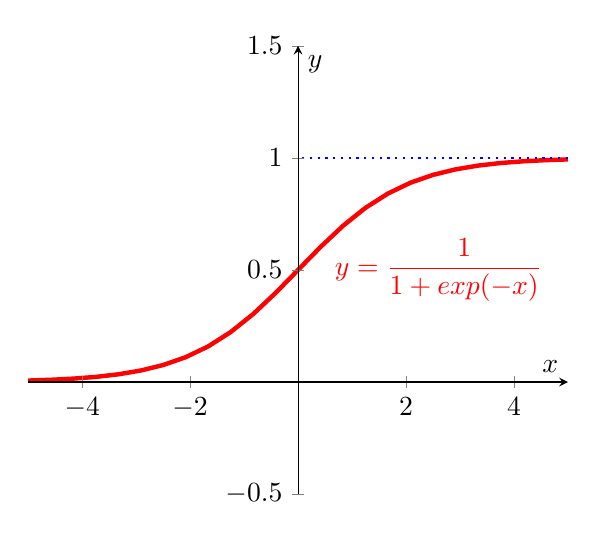
\begin{tikzpicture}
					\begin{axis}[
						xmin=-5, xmax=5,
						ymin=-0.5, ymax=1.5,
						axis lines=center,
						axis on top=true,
						domain=-5:5,
						ylabel=$y$,
						xlabel=$x$,
						]

						\addplot [mark=none,draw=red,ultra thick] {1/(1+exp(-x)};
						\node [right, red] at (axis cs: 0.5,0.5) {$y = \dfrac{1}{1+exp(-x)}$};

						%% Add the asymptotes
						\draw [blue, dotted, thick] (axis cs:+5,+1)-- (axis cs:0,+1);
					\end{axis}
				\end{tikzpicture}}
		\end{column}
	\end{columns}
\end{frame}

%%%%%%%%%%%%%%%%%%%%%%%%%%%%%%%%%%%%%%%%%%%%%%%%%%%%%%
%%%%%%%%%%%%%%%%%%%%%%%%%%%%%%%%%%%%%%%%%%%%%%%%%%%%%%
\subsubsection{Transfer Functions}
\begin{frame}{Transfer Functions - tanh}
	\begin{columns}
		\begin{column}{0.5\textwidth}
			\begin{itemize}
				\item In practice its preferred over the sigmoid activation since it is zero centered.
				\item The activations still saturate (therefore killing the gradient).
				\item It is effectively a scaled sigmoid $\rightarrow tanh(x) = 2 \sigma(2x)-1$.
			\end{itemize}
		\end{column}
		\begin{column}{0.5\textwidth}
			\resizebox{\textwidth}{!}{
				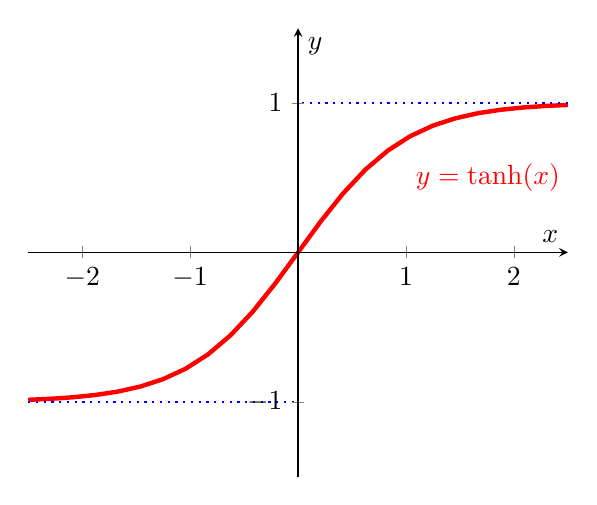
\begin{tikzpicture}
					\begin{axis}[
						xmin=-2.5, xmax=2.5,
						ymin=-1.5, ymax=1.5,
						axis lines=center,
						axis on top=true,
						domain=-2.5:2.5,
						ylabel=$y$,
						xlabel=$x$,
						]

						\addplot [mark=none,draw=red,ultra thick] {tanh(\x)};
						\node [right, red] at (axis cs: 1,0.5) {$y = \tanh(x)$};

						%% Add the asymptotes
						\draw [blue, dotted, thick] (axis cs:-2.5,-1)-- (axis cs:0,-1);
						\draw [blue, dotted, thick] (axis cs:+2.5,+1)-- (axis cs:0,+1);
					\end{axis}
				\end{tikzpicture}}
		\end{column}
	\end{columns}
\end{frame}

%%%%%%%%%%%%%%%%%%%%%%%%%%%%%%%%%%%%%%%%%%%%%%%%%%%%%%
%%%%%%%%%%%%%%%%%%%%%%%%%%%%%%%%%%%%%%%%%%%%%%%%%%%%%%
\begin{frame}{Transfer Functions - relu}
	\begin{columns}
		\begin{column}{0.5\textwidth}
			\begin{itemize}
				\item Easy to compute and doesn't saturate.
				\item Found to greatly accelerate backpropagation.
				\item Unfortunately ReLU units can be fragile during training: A large gradient may knock the unit out of the data manifold.
				\item Usually works better than the others (if you're careful).
			\end{itemize}
		\end{column}
		\begin{column}{0.5\textwidth}
			\resizebox{\textwidth}{!}{
				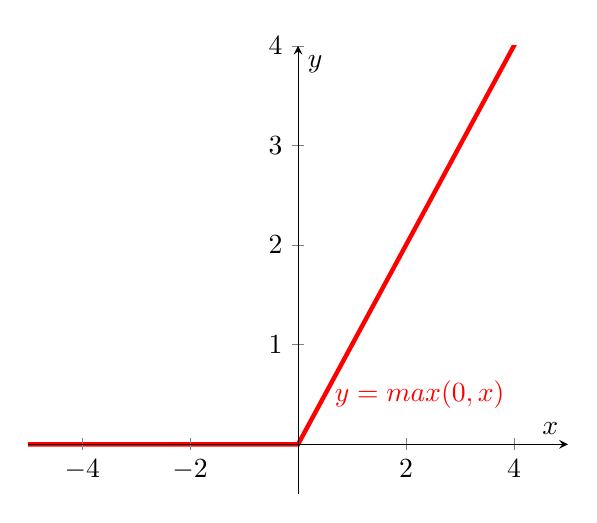
\begin{tikzpicture}
					\begin{axis}[
						xmin=-5, xmax=5,
						ymin=-0.5, ymax=4,
						axis lines=center,
						axis on top=true,
						domain=-5:5,
						ylabel=$y$,
						xlabel=$x$,
						]
						\addplot [mark=none,draw=red,ultra thick] {x*(x>0)};
						\node [right, red] at (axis cs: 0.5,0.5) {$y = max(0, x)$};
					\end{axis}
				\end{tikzpicture}}
		\end{column}
	\end{columns}
\end{frame}

%%%%%%%%%%%%%%%%%%%%%%%%%%%%%%%%%%%%%%%%%%%%%%%%%%%%%%
%%%%%%%%%%%%%%%%%%%%%%%%%%%%%%%%%%%%%%%%%%%%%%%%%%%%%%
\subsection{Training}
\begin{frame}{Weight Initialization}
	\begin{itemize}
		\item Weight initialization becomes very important!
		\item \textbf{Not} all zeros!
		      \begin{itemize}
		      	\item If all the weights are zero, they can only change in the same direction and by the same amount.
		      \end{itemize}
		\item \textit{Small} random numbers.
		      \begin{itemize}
		      	\item Not \textbf{too} small, as that may cause the gradients to be too small.
		      	\item Called "symmetry breaking" - avoids the problem of weights changing in the same way.
		      	\item Some heuristics might be helpful (Xavier Initializer - weights are initialized based on the fan-in, fan-out and activation function - \textit{tf.contrib.layers.xavier\_initializer()})
		      \end{itemize}
		\item Bias can be set to zero.
		      \begin{itemize}
		      	\item Symmetry breaking provided by weight initialization
		      \end{itemize}
	\end{itemize}
\end{frame}


%%%%%%%%%%%%%%%%%%%%%%%%%%%%%%%%%%%%%%%%%%%%%%%%%%%%%%
%%%%%%%%%%%%%%%%%%%%%%%%%%%%%%%%%%%%%%%%%%%%%%%%%%%%%%
\subsection{Code Example}
\begin{frame}{Code Example}
	\begin{center}
		\textcolor{blue!75}{\underline{ \href{https://github.com/davifrossard/iml/blob/master/04_LogRegAndNN/Sample_Code/Neural Network.py}{External Code}}}
	\end{center}
\end{frame}

%%%%%%%%%%%%%%%%%%%%%%%%%%%%%%%%%%%%%%%%%%%%%%%%%%%%%%
%%%%%%%%%%%%%%%%%%%%%%%%%%%%%%%%%%%%%%%%%%%%%%%%%%%%%%
\begin{frame}{Learned Weights}
	\begin{center}
		\includegraphics[width=0.9\columnwidth,trim={0 0 0 1cm},clip]{nn_weights}
	\end{center}
\end{frame}


\end{document}
